\chapter{Iterations}
This chapter chronicles the development in a diary format. Iterations were used during the development of this project, with each iteration typically consisting of at least one story and often included non story based work. However, due to the iteration process, each story consisted of analysis, design, implementation and testing. Therefore, each of these bits of work are given within the iteration they were completed in, negating the need for an initial design section.

\section{Outline}
TODO: could this be past tense instead?
\begin{enumerate}
	\item Iteration 0 mostly involves the setting up of the tools to be used in the project, some research and the creation of an initial database design.
	\item Iteration 1 is concerned with the implementation of the database design and setting up the initial admin area with a list of quizzes owned by the admin who logged in.
	\item Iterations 2 focusses on the creation of quizzes by admin users.
	\item Iterations 3, 4 and 5 involves the implementation of running sessions.
	\item Iteration 6 focusses on the submission of answers and displaying results. It also deals with the security issue from Qwizdom.
	\item Iteration 7 involves making the application mobile responsive, the part two redesign which led to implementation of the the way slideshows could be run on the application.
	\item Iteration 8 is only concerned with report writing.
	\item Iteration 9 contains security testing, more report work, the server setup , and bug fixing.
	\item Iteration 10 is the last iteration and followed the final bits of report writing, the user testing, and the implementation of downloading results and various bug fixes.
\end{enumerate}

\section{Tools used}
There were a number of tools used throughout development that do not fit under a single iteration. The main three were a Wordpress diary, a Trello board and Git. 

The diary was used to keep track of the major pieces of development done each week and any questions/ issues that needed to be raised during supervisor meetings. This was a simple Wordpress site that was set up several years ago and repurposed for the use in this project.

Trello is a project management tool that allows users to create a "board" for a project that then allows the creation of cards that tasks can be added to\cite{trello}. Feature tracking is a key part of the system as tasks and cards can be marked as complete, Trello suits XP based approaches as cards can be created and edited on the fly for each iteration. For this project, a card was created for each iteration, with a list of stories and tasks to be completed within that iteration. Once a task was completed, it was checked as such giving an easy to read percentage completion for the story. See \ref{fig:trello-board} below for an example of the board used in this project.

\begin{figure}
	\caption{Part of the Trello board used for this project, showing a few iterations and the high level tasks within them.}
	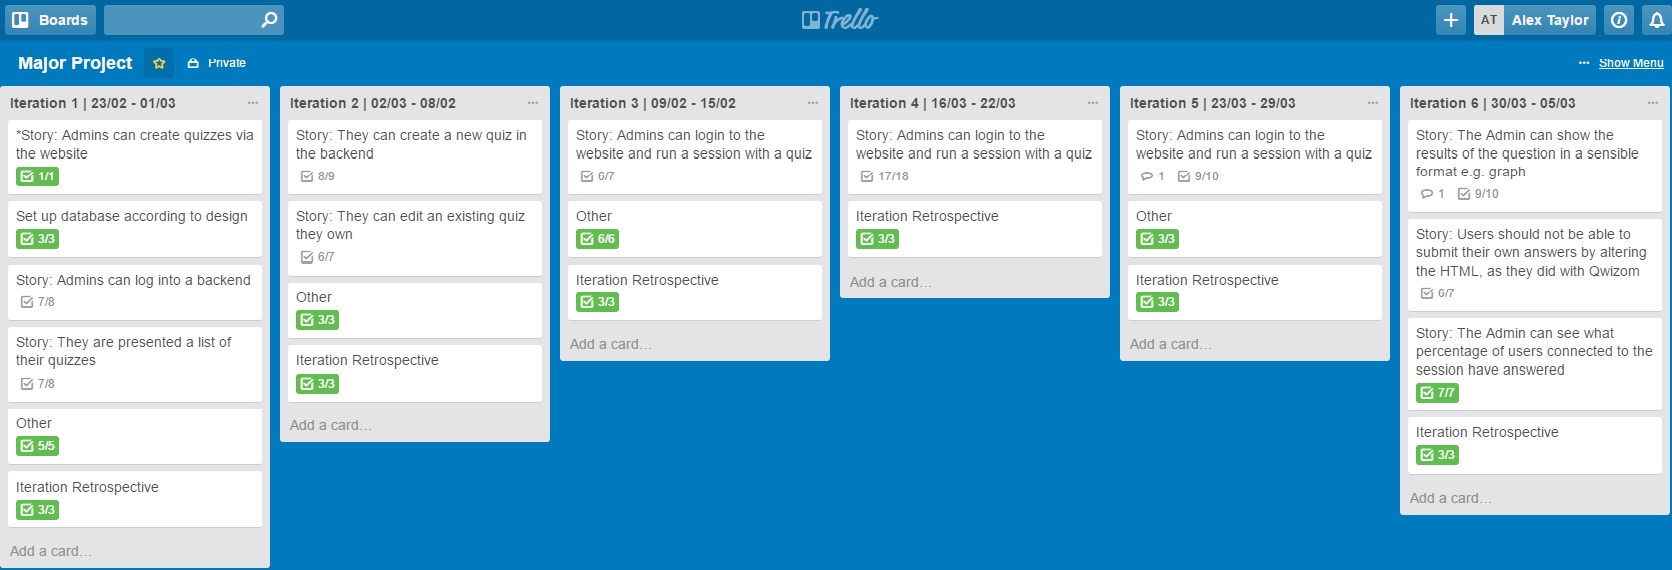
\includegraphics[width=\textwidth]{Chapter2/trello-board}
	\label{fig:trello-board}
\end{figure}
\newpage

Git was used extensively during development, primarily for version control but also a form of backup and as an easy way to deploy the system. Version control is very important as it allows tracking changes to the project and if a mistake it made, can be used to undo these mistakes. It also allows branching out bits of functionality, so developing features can be done separate from the rest of the project and once working, merged back in. Github was used as the repository service due to it being free and easy to use\cite{github}.

Laravel comes with a custom Command Line Interface, CLI, called Artisan\cite{artisan}. Artisan is used to run the majorty of commands needed in Laravel, from the migrations to the creation of controllers. An example would be \textit{php artisan migrate} which migrates the database. It is always prefixed with "php".

The last main tool used was Microsoft Visio\cite{visio} which was used to create the majority of diagrams in the design sections of the report.

As well as tools, three online sources were used extensively. The first is Laravel Recipes, which provided a number of examples of how to use helpers and facades\cite{laravel-recipes}. The second, Laracasts, an online Laravel tutorial site, especially the Intro to Laravel series\cite{laracasts}. And finally, the documentation pages\cite{laravel-docs}.
\newpage

\section{Iteration 0 16/02 - 22/02}
\subsection{Initial work}
This iteration did not consist of any development. It consisted mainly of research and design work. But most importantly it included writing the stories for the project. 

Other items of work involved setting up a diary, a Trello board for documenting all the work and setting up the initial Git repository along with linking it to Github.
\subsubsection{Research}
Research was focussed on several areas, and some documents were produced from this research. The first area of research was on the frameworks available, after which Laravel was selected. Hosting options were also explored and a document discussing both of these was produced, this document will form part of the Background chapter when it comes to writing the report.

Some additional research was also completed on the Microsoft PowerPoint Add-In for the second part of the project. This was mainly to get a sense of the amount of work involved, and what language/ environments would be needed. This research did not go into much depth as further research will be undertaken when that part of the work is reached.
\subsubsection{Design}
The design work completed was a database design. This would be needed throughout the whole project so made sense to write initially, though it may be subject to significant changes. Figure \ref{fig:initial-er-diagram} is the ER diagram.

\begin{sidewaysfigure}
	\caption{Entity relationship digram for the initial database}
	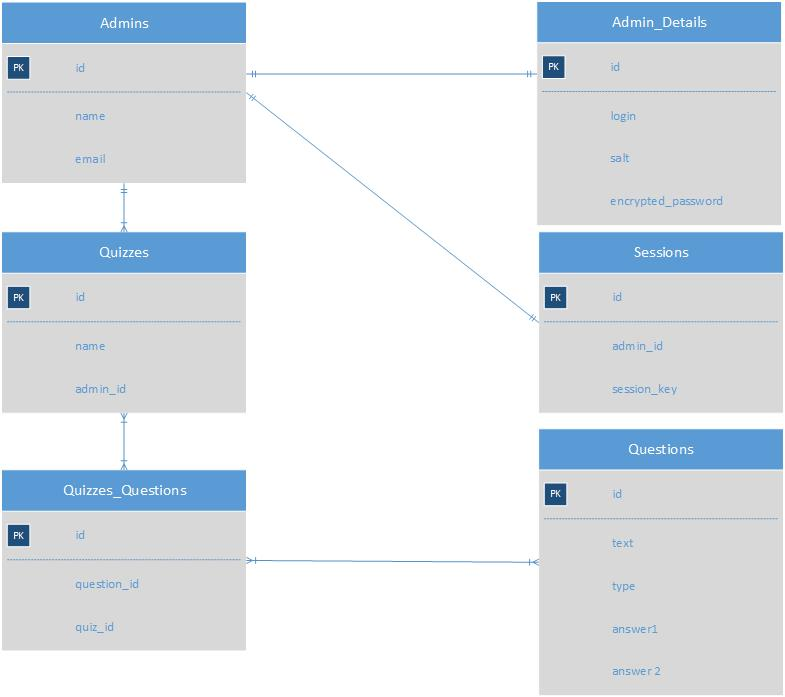
\includegraphics[width=\textwidth]{Chapter2/Iter-0/Initial-ERDiagram}
	\label{fig:initial-er-diagram}
\end{sidewaysfigure}

\subsubsection{Stories}
A list of stories was produced and written up in a separate document. These stories will be the basis of the project and act as the functional requirements for the evaluation at the end of development (appendix \ref{appendix:initial-stories}).
\newpage

\section{Iteration 1 23/02 - 01/03}
\subsection{Story: Admins can create quizzes via the website}
\subsubsection{Analysis - Breakdown of Tasks}
This story is quite large and should be broken down into several substories:
\begin{itemize}
	\item (3) Admins can log into a backend
	\item (2) They are presented a list of their quizzes
	\item (5) They can create a new quiz in the backend
	\item (3) They can edit an existing quiz they own
\end{itemize}
These have been added to the story list document.
\newpage

\subsection{Story: Admins can log into the backend}
\subsubsection{Analysis - Breakdown of Tasks}
\begin{itemize}
	\item Create users table
	\item Add login page
	\item Add register page
\end{itemize}
\subsubsection{Design}
Design was limited due to the automated builder. However it added some view files and a default HomeController for a basic homepage.
\subsubsection{Implementation}
Implementing this was far easier than originally anticipated, Laravel comes with the needed tables out of the box and has a command to run that sets up simple auth for users: \textit{php artisan make:auth}
\subsubsection{Testing}
Because the login and auth is handled by Laravel by default, testing it was deemed to not be a priority. However, three simple tests were written to ensure it never breaks due to future changes. Dusk Tests:
\begin{enumerate}
	\item Test to ensure the application redirects to /login is the user is not already logged in
	\item Test for logging in with a user in the database
	\item Test for registering a new user
\end{enumerate}
\newpage

\subsection{Story: They are presented a list of their quizzes}
\subsubsection{Analysis - Breakdown of Tasks}
\begin{itemize}
	\item Make the homepage the QuizController rather than the HomeController
	\item Check and get the user who is logged in
	\item Display a list of quizzes for that user
\end{itemize}
\subsubsection{Design}
The HomeController to be removed in this period of work and the QuizController used in its place. (TODO: Digitize UI mock)
\subsubsection{Implementation}
Quite an easy amount of work, changing the controller was a simple change to the routes and then updating the quiz view file to use the same layout as the original home views. To get the user, a helper function is provided: \textit{auth()-$>$user()} which gets the user object. Obtaining the id from this is simple and then using an Eloquent ORM call it is easy to find all the quizzes owned by that user.
\subsubsection{Testing}
Dusk tests for this story:
\begin{enumerate}
	\item Test to see if the /home page lists the quizzes as it would on the /quizzes page
	\item Test to see if a quiz that belongs to a user is present on the page
	\item Test to see if a quiz that belongs to another user is not present on your page whilst your own is
\end{enumerate}
These tests highlighted a problem with the testing framework however. Chrome is used as the Remote Web Driver for running these application tests in. For each test a new migration is made within the test database, thereby wiping the data created within each test. An unintended side effect however is that every new user created starts at id=1 in the users table (a user has to be created for all these tests.) The Chrome driver seems to remember that the user of id=1 logged in, in the previous test and therefore skips the auth step. This means the test order is messed up due to the test trying to log in even though it is already logged in. The solution to this is to create each new user in the next id record, whilst this is somewhat convoluted, it seems to work.

Potential future tests: Use sessions have two users log in and see/ not see the relevant quizzes.
\newpage

\subsection{Non-Story Work}
\subsubsection{Database Work}
Some initial work that is needed for almost all the stories is having a working database set up to store the users, quizzes, questions etc. Seeing as the amount of work to setup all the tables and their relationships would not take long, it was decided that this could be done all at once at the start of the iteration.

While creating these tables it was possible to create the controllers needed within the application at the same time using: \textit{php artisan make:model *name* -mc } 
\subsubsection{Seed Data}
Because of the amount of changes to the database that were being made, the tables were repeatedly wiped and seeding some data was needed. To do this some seeders were generated with \textit{php artisan make: seed *name*}. These were created under database/seeds/ and simply required creating new objects of the desired Model and adding the various fields as parameters of the objects. These objects are then saved to the database. These seeders can be run when a migration is called such that the data is replaced as soon as its lost.
\subsubsection{Layout Changes}
The initial \textit{make:auth} command created a default home page with a menu bar and some basic styling. This styling was created with Bootstrap and looks quite nice so the basic styling has been kept. This layout was modified somewhat to add some menu options that persist across pages. This layout is then used by all the backend pages created by extending it.
\newpage

\subsection{Review and restrospective}
\subsubsection{Review}
Completed stories with their associated difficulties in parenthesis:
\begin{enumerate}
	\item (6) Admins can create quizzes via the website
	\item (3) Admins can login to a backend
	\item (2) They are presented a list of their quizzes
\end{enumerate}
The first story was quite large so was split up, thus making it quite an easy task with no problems.

The second and third were not that challenging either, two in particular was made much easier thanks to the built in auth builder from Laravel. This means that the rating of three is wrong and it should be lower at a one. Story three fits a difficulty of two as it provided no major problems, but it did give ample opportunity to learn Laravel much better. For example learning the structure and how to use helper functions such as the one to get the currently authenticated user.

All implementation tasks were completed, but some documentation for story two and three was missed. That is to be completed at the start of the next iteration.

\subsubsection{Retrospective}
Breaking the stories up into substories and then those stories into subtasks is very useful for the project. It splits the functionality well allowing individual components to be built and showcased on the development site.

However, the documentation did not go well. A majority of the design, testing and implementation documentation was missed during the iteration. This was mostly due to overestimating the amount of time available to write this. In further iterations, more emphasis should be placed the documentation section of work.
\newpage


\section{Iteration 2 02/03 - 08/03}
\subsection{Story: They can create a new quiz in the backend}
\subsubsection{Analysis - Breakdown of Tasks}
\begin{itemize}
	\item Need quiz/new form to add name
	\item Add validation
	\item This then redirects to quiz.show for this new quiz
	\item This page needs a button that can add a question
\end{itemize}
\subsubsection{Design}
The design is split into two parts, design for the quiz/new page and a design for the question/new page:
(TODO: digitise images for these)
Use case at this point \ref{fig:quiz-create-use-case}
\begin{figure}
	\caption{Use case diagram for the admin backend with create quiz functionality}
	\centerline{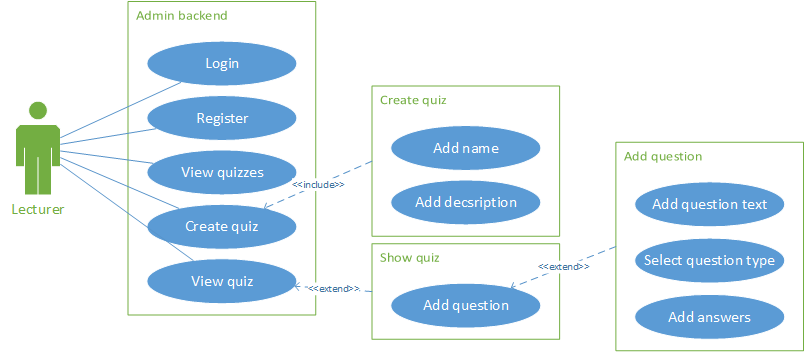
\includegraphics{Chapter2/Iter-2/iter-2-use-case-create}}
	\label{fig:quiz-create-use-case}
\end{figure}
\subsubsection{Implementation}
A create page was added for quizzes, this was linked to from the home page. This was mapped to /quizzes/create address. A simple form was added to this page with the name and description of the quiz. Questions would be added on an individual quiz page. The form sends the form as an HTTP POST request to the /quizzes page which then maps onto the 'Store' action in the Quiz Controller. This action is used for server side validation and saving the data to the database using an Eloquent function. This Eloquent function also returns the id of the new quiz. The user\_id is assigned to the quiz by simply getting the current user. Using this id, this Store function redirects to the newly created quiz.

On a quiz page, it displays the name and description and has a button to add any questions to the quiz. This button links to the questions/create page that functions in the same way as the quiz creation, albeit with the relevant fields in the form. The questions are assigned to the quiz by passing the quiz id to the question creation page in a GET variables via the url. This allows the question to be assigned to the quiz during its creation in the database and to be redirected back to the quiz page.

For validation there are two parts, one on the HTML form and the other handles server side. The HTML validation (client side) uses simple HTML 5 validation like the "required" attribute in the form inputs. Further frontend validation could be added utilising JavaScript but the HTML solution was far easier to implement, being the addition of one word and not several lines of code that have to be built and added to the correct pages. The server side complements this as client side validation can be circumnavigated by determined users.

The server side validation in Laravel is well supported and made as easy as possible to implement. The Store function used to save data from the POST request simply calls \textit{\$this-\textgreater validate()} on the request data. Inside this validation function, various rules can be imposed on individual pieces of the request data such as simply requiring that is is filled or that it has to have a minimum length\cite{laravel-validation}.

Something that Laravel enforces is the use of CSRF tokens to prevent cross site request forgery attacks on the site. A token is generated for the project during its creation, and this token must be placed in a hidden field within every form so that it can verify that the authenticated user is the one actually making the requests to the application\cite{laravel-csrf}.
\subsubsection{Testing}
Dusk tests:
\begin{enumerate}
	\item Test to create a new quiz
	\item Test the HTML validation for creating a new quiz
	\item Test backend validation of quizzes
	\item Test a quiz contains questions that have all been added before hand
	\item Test to add a question to a quiz
	\item Test to make sure the question page contains the relevant information
\end{enumerate}
A problem encountered in this set of tests is the speed of testing. Running these tests takes about a minute. The reason for this is that the tests use DatabaseMigrations rather than DatabaseTransactions, meaning that the database is migrated for every test. Using transactions would reduce the time taken by only doing a migration at the start and then using a transaction for each test. Alternatively having a pre migrated test database on which you run transactions would work too, but this would mean any time you change your database, you would have to remember to migrate the test database. 

After attempting to use the transactions it appears as though they are not usable within Dusk. This is because Dusk is running in another process and migrations is the only choice\cite{dusk-transactions}. 
\newpage

\subsection{Story: They can edit an existing quiz they own}
\subsubsection{Analysis - Breakdown of Tasks}
\begin{itemize}
	\item There is an edit button on quizzes that links to quiz/edit
	\item You can edit the name of the quiz
	\item You can remove questions
	\item You can add questions
	\item You can edit the content of a question
	\item You can delete a quiz and its associated questions
\end{itemize}
\subsubsection{Design}
There was not much design for this stage as it only really adds an edit page which should look the same as the create pages in the above story except that the input fields are pre-filled with data that is being editing. Additionally a delete button should be added for quizzes and questions. (TODO: more design here) Figure \ref{fig:quiz-edit-use-case}
\begin{figure}
	\caption{Use case diagram for the admin backend with edit quiz functionality}
	\centerline{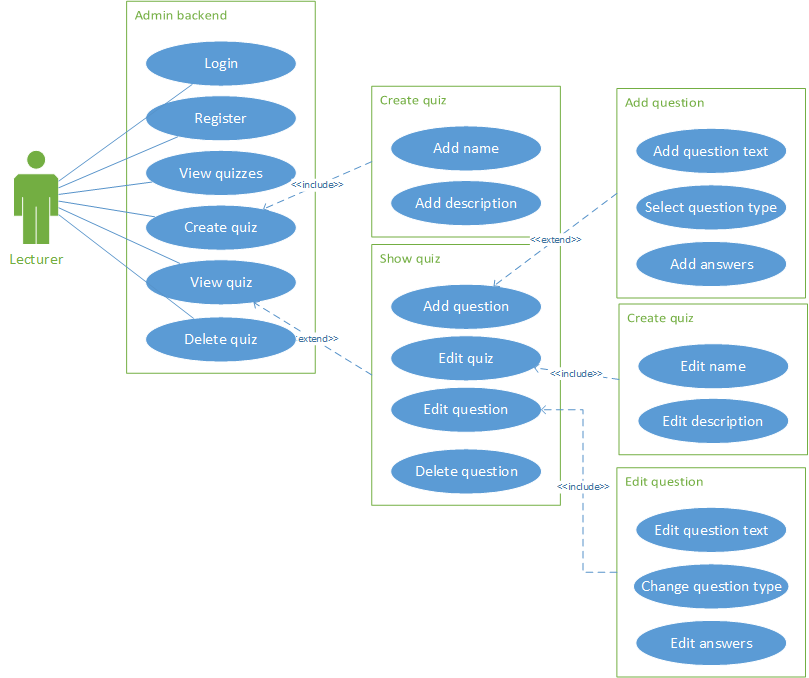
\includegraphics{Chapter2/Iter-2/iter-2-use-case-edit}}
	\label{fig:quiz-edit-use-case}
\end{figure}
\subsubsection{Implementation}
Pre filling the edit page was done by getting the record in the database by the id and just setting the default values of the input fields. The main difference to the creation stage was that the form had to use the HTTP PATCH method rather than POST. This PATCH method is automatically routed to the update function in the controller\cite{laravel-resource-controller}. Within this function, server side validation is performed and and Eloquent called to update the row in the database. It then redirects back to the quiz page for editing either a question or quiz.

Delete buttons were added to the quizzes and questions, these were not a simple \textless a \textgreater tag that linked to a delete page like the create and edit pages. This had to be a small form that sent an HTTP DELETE request along with an id to the /quizzes or /questions page. This was mapped to the destroy functions in the respective controllers which simply called an Eloquent function that removed the record. Due to the way the database is designed when a quiz or question is deleted, the linking row inside the quiz\_question table must also be deleted. 

Another thing that had to be changed was to make the foreign key reference columns in the quizzes and questions table cascade delete on deletion of the record. This meant that they would delete the rows in the quiz\_question table that referenced the row being deleted. For a quiz deletion, this had to go further and also find the questions associated with the quiz and delete all of those, which used a simple Eloquent function to find them using the quiz\_question table before the rows in that table were deleted and then delete the questions using those ids. 
\subsubsection{Testing}
Dusk Tests:
\begin{enumerate}
	\item Test the deletion of a quiz
	\item Test the deletion of a question on a quiz
	\item Test the edit page of a quiz
	\item Test the edit page of a question
\end{enumerate}
\newpage

\subsection{Non-Story Work}
\subsubsection{Seeding}
Some more data needed to be seeded for this subsection of work, the question data. This involved creating some new Model Factories and using them in the seeders correctly. One issue was trying to create many questions for individual quizzes, but this was overcome using some very basic looping and calling the model factories in the right places.
\subsubsection{Quiz Description}
It was decided that quizzes should probably have descriptions attached to them, in case the lecturer needs reminding of what it is in 6 months time. This involved creating a new migration and simply adding a column to the table.
\subsubsection{Travis Setup}
Travis is a CI tool that can be used to run tests automatically on git pushes. Setting it up involved doing some spike work with another git project. It is really easy to set up, needing you to simply add a travis.yml file which specifies what Travis will do after a push. The project also has to be added from Github which is simple.
\newpage

\subsection{Review and restrospective}
\subsubsection{Review}
\begin{enumerate}
	\item (5) Admins can create a new quiz in the backend
	\item (3) They can edit an existing quiz they own
\end{enumerate}
The difficulty ratings were accurate, with the work taking about the expected amount. Some of the extra work here involved trying to set up Travis for continuous integration which could be used for running tests automatically was somewhat problematic but did not take up too much time. These stories were almost fully completed with the exception of some testing as described below.

\subsubsection{Retrospective}
The documentation stage improved this iteration compared to the last, even with the added responsibility of finishing documentation from the week before.

Unfortunately, testing took a hit, this is mainly due to the attempted use of test driven development. This practice was originally done to try and improve the code quality. However the nature of a web application and the use of a large framework is problematic for TDD. Trying to write tests for all the various parts of the web application is hard, and the framework also does a lot of work for you, so writing things like unit tests beforehand is hard. Application tests using Laravel Dusk are more appropriate but they test the story itself rather than underlying logic, which is less applicable to TDD. 

To mitigate the lack of tests written in future, TDD will be dropped due to the above reasons.
\newpage


\section{Iteration 3 09/03 - 15/03}
\subsection{Story: Admins can login to the website and run a session with a quiz}
\subsubsection{Analysis - breakdown of tasks}
This story is quite large and whilst it will probably be split into a number of tasks, the first thing to do was some spike work on the way this system would work. One route is with WebSockets, a relatively new technology that allows the server to push data to the page quickly and easily\cite{websockets}. This would be nice solution as it is relatively future proof and seems like a better alternative to other solutions that involve a lot of JavaScript and forcing page changes on the users.
\subsubsection{Design}
WebSockets were introduced into Laravel 5 and have become one of the defacto ways to update the front end in real time. Unlike in some other web frameworks such as Ruby on Rails the web sockets in Laravel requires some extra set up. In Rails the WebSockets can be run on the main web server that is used to run the site\cite{rails-websockets}, in Laravel however another server has to be set up to run these. Laravel offers several different drivers for running the WebSockets, including a Redis server and a third party application called Pusher\cite{laravel-broadcasting}. Pusher handles most of the work for you and requires little set up other than creating a free account\cite{pusher-what-is}.
\subsubsection{Implementation}
Pusher was chosen due to its ease of use and due to its high recommendation rate within the Laravel community. A problem with Pusher is that due to it being a third party service, it is not free forever (it has a number of users limitation). However you could host your own Redis server to mitigate this cost. This means that the system had to be designed in a way that the driver for WebSockets could be changed with ease.

After configuring the spike work application to use Pusher, a simple Laravel Event was created to send a message to the Pusher. To test this event there were a couple methods implemented. The first was to simply register a route that triggers it when the page is visited. (TODO: show an example of an event call?)
 
Or with a custom made artisan command that can trigger the event: php artisan quiz:send {message}. A command is very useful for testing the event as it can be used without building a button on the front end to trigger it.

Two online guides were used to help write this section of the system due to WebSockets being a new technology\cite{pusher-guide}\cite{echo-guide}. Though they were used to get the basic concepts working, the final code used within the project is tailored to the system and is therefore different overall.
\subsubsection{Testing}
There was no testing as it was spike work.
\newpage

\subsection{Non-story work}
\subsubsection{Refactor controllers}
The first major piece of work was to refactor the controllers and models into a far more sensible structure. The problem was that the Eloquent functions for modifying and reading from the database was within the controllers. In a full MVC system, this functionality should be inside the models. To fix this, the Eloquent functions were refactored into the respective quiz and question models. This would make it easier if anything ever needed to change within the logic for any database interactions.
\subsubsection{Changing the DB structure}
The original design was changed, and the quiz\_questions table for linking quizzes and questions together was removed. The original reason for this table was most likely such that questions could be reused. However, after thinking about the potential for that to happen, and the issues that the structure was causing in the model logic it was decided that the quiz\_question table was more of a hindrance than a help.

The questions table now simply has a quiz\_id column that references the quiz it belongs to. Doing this means that the relationships between the two tables are much easier to define in the models, simply having a belongsTo and hasMany function in both that automatically return the necessary data. Thanks to the previous refactoring of model logic, changing this functionality was quite quick. Deleting rows in the database was also simpler now that there was no quiz\_questions table, all the related questions when a quiz is deleted can be deleted at the same time using the onDelete cascade property in the database.
\subsubsection{Front-end setup}
This was the first time that any custom CSS was written and Laravel uses SASS to generate its CSS. To build this SASS into CSS, and also to build any future JavaScript, Laravel Mix was needed to run builds for this code. For this, npm and node had to be installed so that they could run their Webpack build scripts. There were some issues trying to get the build scripts to run, even though it worked on fresh installs of Laravel, but eventually a Github issue was discovered that had some solutions\cite{broken-mix}.
\subsubsection{Dusk and travis}
The aim was to try and set up Laravel Dusk on Travis. Dusk can use a few different browser drivers for running the tests in, by default this is Chrome but Travis comes preconfigured with PhantomJS which is also supported by Dusk. It should be a simple swap in drivers and then to set Travis to run a PhantomJS server. Unfortunately this does not seem to work, and no reason can be found. A supposedly working copy was even cloned and that does not work for therefore it has to be concluded it is currently not working.
\newpage

\subsection{Review and restrospective}
\subsubsection{Review}
No actual story work was completed, however a large amount of non story work was completed. Additionally a large amount of spike work was completed for the story: Admins can login to the website and run a session with a quiz

There was a significant amount of refactoring in this iteration which was not too challenging. The most problematic bit was trying to get the database migrations done properly.

The spike work was particularly challenging this week because it was attempting to work with a new technology. It also involved the use of various parts of the Laravel framework not encountered before, like events and writing custom artisan commands.

\subsubsection{Retrospective}
The spike work was very useful for the overrall devlopment of the application. Additionally the refactoring and restructing of the database and testing has helped a lot with the future outlook of the application.

A negative was the continuous integration on Travis. Laravel Dusk is a relatively new testing framework and Travis does not seem to work well with it. This means that the tests written cannot be run on Travis. It therefore makes CI somewhat pointless if the tests cannot be run and this will be left for now.
\newpage


\section{Iteration 4 16/03 - 22/03}
\subsection{Story: Admins can log into the website and run a session with a quiz}
\subsubsection{Analysis - Breakdown of Tasks}
After doing some spike work last week, this task can now be approached and broken into several sub tasks:
\begin{itemize}
	\item Set up config for Pusher
	\item Add event for broadcasting
	\item Write a command to trigger this event
	\item Add a button to quizzes to trigger this event
	\item Display this on the front end using the JavaScript which listens for Pusher events
	\item Add a session key box to front page
	\item Add session id to users
	\item Allows admins to change their id
	\item When admin clicks run, this id can be entered into the key box to join a channel with the name of the id
	\item The user will be presented with the initial quiz page which will be default filled with the name and description of the quiz
	\item The admin will see the same page but with an "admin panel"
	\item This admin panel has a next and previous button for questions
	\item When these buttons are pressed, the question is sent to pusher
	\item These question are rendered as a form on the user end and admin end
	\item The user can submit the form
\end{itemize}
\subsubsection{Design}
Mockups of the student end of the system: 
\begin{center}
	\begin{figure}
		\caption{Design for a quiz on a desktop}
		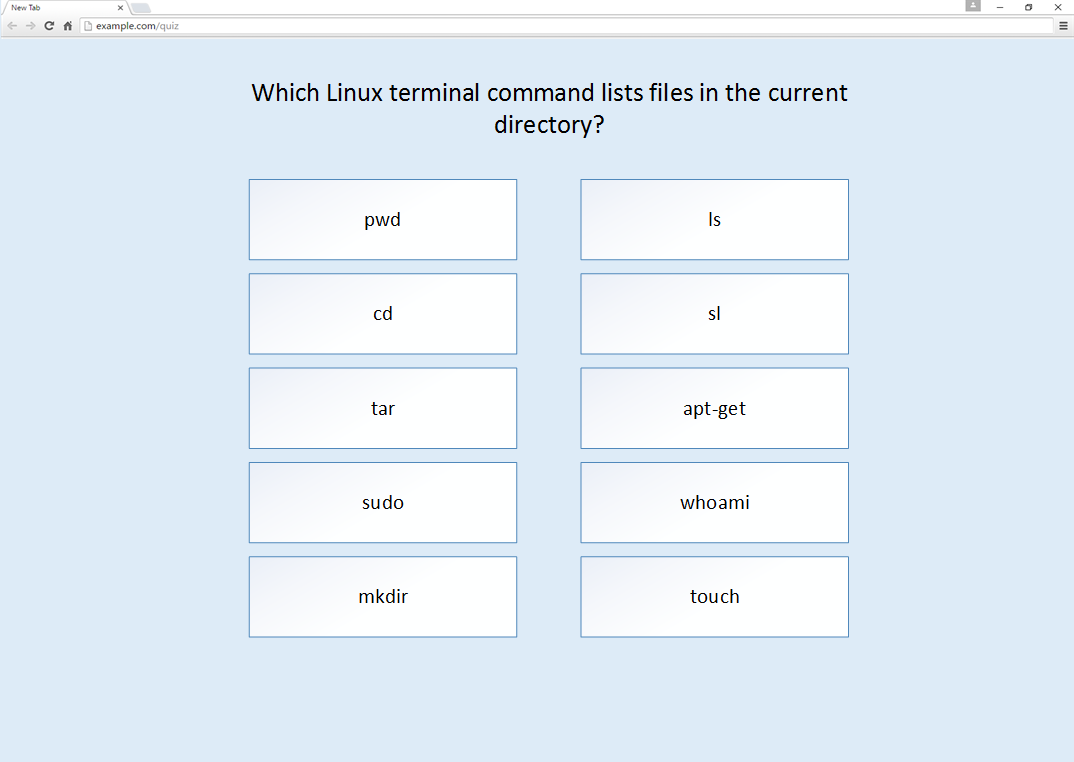
\includegraphics[width=\textwidth]{Chapter2/Iter-4/Quiz-Web-Design-Cropped}\\
		\label{fig:quiz-desktop}
	\end{figure}
	\vspace{1cm}
	\begin{figure}
		\caption{Design for a quiz on a mobile device}
		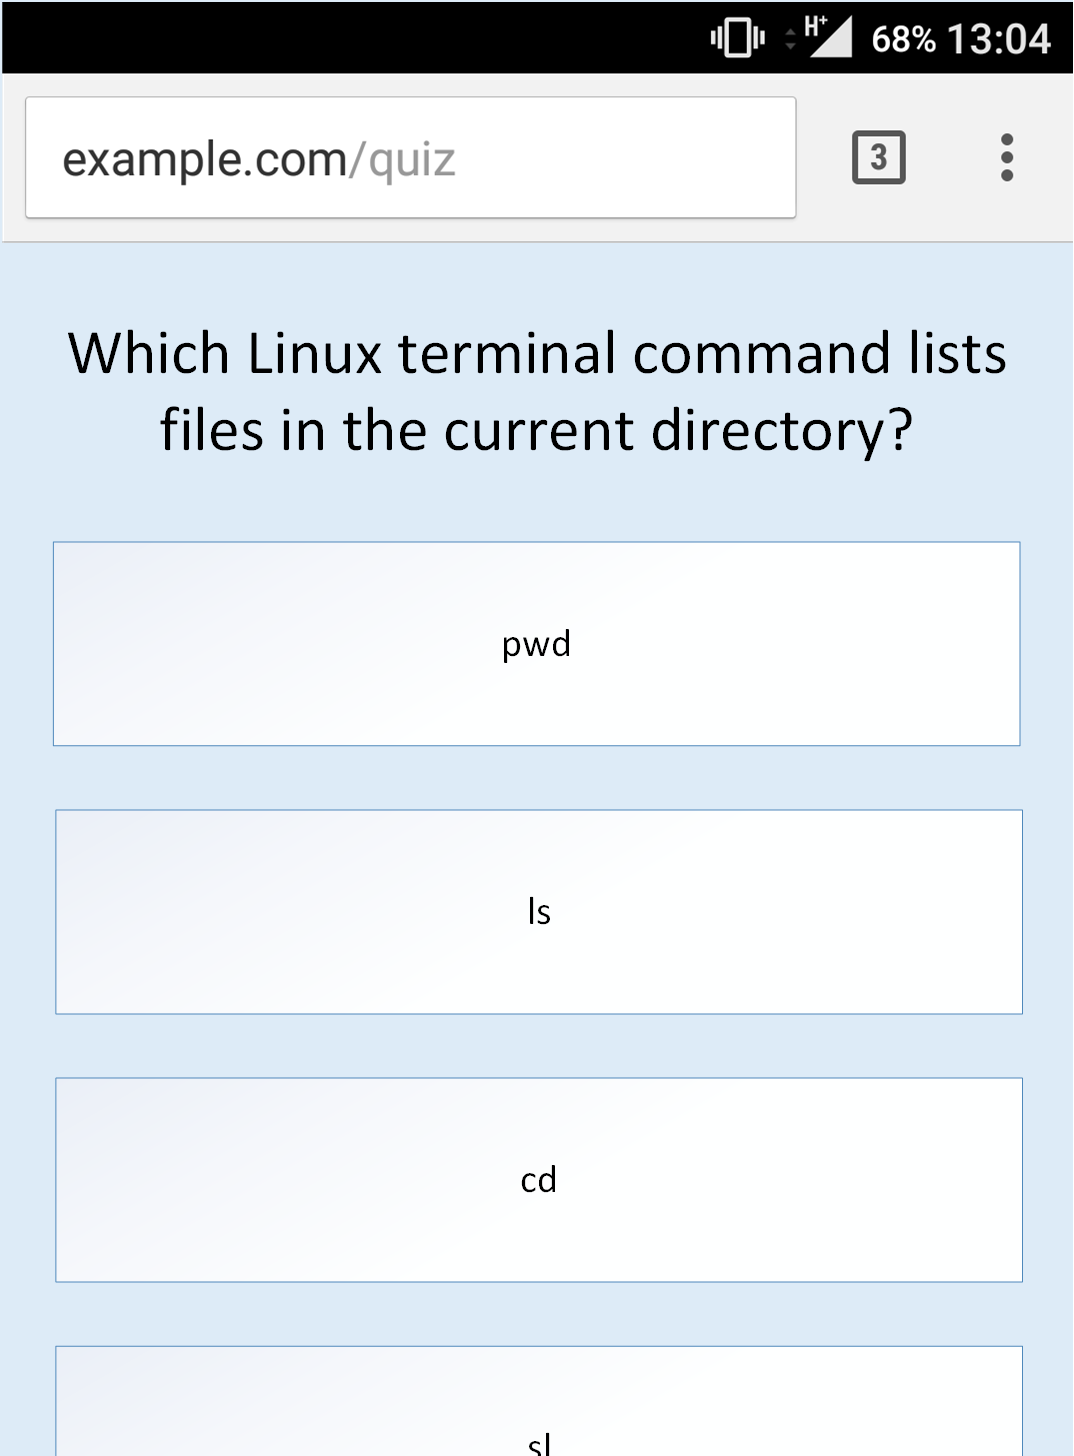
\includegraphics[scale=0.25]{Chapter2/Iter-4/Quiz-Mobile-Cropped}
		\label{fig:quiz-mobile}
	\end{figure}
\end{center}


\subsubsection{Implementation}
It began by configuring pusher, creating an event and writing some basic JavaScript to append to the front page. Some work was done on the admin panel as well, making it only visible to logged in users (the lecturer running the quiz), and adding the functionality for previous and next question buttons. These are buttons that send AJAX requests to quiz controller actions which then trigger the event for WebSockets with the appropriate question data.

Early into the iteration a major flaw with using the WebSockets came up, whilst new content was easy to add to the page, if a new user joined the session late, they would see a blank page/ or the original content of the page that has not yet been removed with JavaScript. To remedy this, the current position in the quiz should be kept track of and the PHP on the page should load the question specified at that position. At the same time, the WebSockets will be running and updating the page from that point onwards in the session. It was decided the best place for keeping track was within the session table, which now has appropriate columns for the position, quiz and if it is running.

Rendering the actual questions calls an action in the question controller, which takes the type of question and the quiz id and position. Using this data it renders one of several available views, one for each type of question like multiple choice or boolean. The views render a simple form showing the question, the possible answers as buttons and a submit button.

For a question to be rendered by default on page load as described above, the page includes the question by rendering the above view. However, it does not know the type of question to render, so it loops over the types and checks if the type of the question is equal to the ones defined earlier in the config file and renders the view if they are the same type. One problem with this is accessing the custom config file. The function to do this was inside the question controller and not the quiz controller. 

Whilst the function could be copied, it was better to create one single helper function that is global to the application. This involved creating a helpers file and adding the function there and then registering the helper function in the composer.json file\cite{laravel-helper-function}.

\subsubsection{Testing}
No testing as the story is not yet complete.
\newpage

\subsection{Review and retrospective}
\subsubsection{Review}
Once again this week no actual story has been completed. This is due to the size of the story and also that some stories are a struggle to work on individually. It seems that the current work covers about six stories rather than just one. Something to not then is that once this piece of work is complete, the velocity will shoot up.

\subsubsection{Retrospective}
The amount of work completed was significant, even if project velocity is 0. But as mentioned this is due to many stories being worked on simultaneously.

However, finishing stories and breaking them up into smaller bits of work that can be finished to give a velocity.
\newpage


\section{Iteration 5 23/03 - 29/04}
\subsection{Story: Admins can login to the backend and run a session with a quiz}
\subsubsection{Analysis - Breakdown of Tasks}
Tasks left over from the previous week:
\begin{itemize}
	\item Form on front page redirects to quiz
	\item Questions rendered as a form
	\item User can submit the form with their answers
	\item Questions need limiting on going above/ below max and min
\end{itemize}
\subsubsection{Design}
\subsubsection{Implementation}
Users still had to connect to the quizzes from the welcome page. A problem with this is that the sessions are being run under the url /quiz/sessionb\_name. This means that submitting a GET or POST form will not work as the url cannot be specified, as the user enters the session key. A solution was to have an input field that took the session key and then used JavaScript to redirect to that session. 

The JavaScript also allowed some client side checking to be done, but there also needed to be server side checks. A custom Middleware class was written to handle the checking of valid session keys. Middleware provide the functionality to filter incoming HTTP requests within controllers\cite{laravel-middleware}. When thr form was submitted, the Middleware function would check the database, and if the requested key was not in the database, would redirect back to the welcome page with an error. Else, it would allow the redirection to the quiz session.

Helper function https://laracasts.com/discuss/channels/general-discussion/best-practices-for-custom-helpers-on-laravel-5?page=2

Issue with Jquery Ajax https://stackoverflow.com/questions/14193469/jquery-is-adding-prevobject-to-array
\subsubsection{Testing}
\subsubsection{Extras}
\newpage

\subsection{Stories Completed}
This iteration and the last have both operated underneath the umbrella of the one story. This is not necessarily accurate as the work that has been completed with this one story covers a multitude of stories. The reason they weren't split up is slightly unclear but part of the reason is the severe overlap between them and some of them being more like functional requirements than areas of work to do. The stories that are now complete:
\begin{itemize}
	\item Multiple different sessions can be run simultaneously
	\item The Admin specifies which question is being run by clicking next/prev question
	\item Sessions can be joined by users via the website
	\item Up to 300 users should be able to join and answer questions (this story is somewhat subjective, but in theory it should scale upwards with no issues)
	\item Users answer the question being displayed by the quiz
\end{itemize}
\newpage

\subsection{Non-Story Work}
\subsubsection{User Page}
A large amount of work was done on the user pages, this was to ensure that admin could view and edit their details including changing their session keys. This work was rather simple and just involved creating the user blade pages, adding the various functions to the controller and model and adding a little bit of functionality to the authentication actions for registering a new user.
\subsubsection{JavaScript Clean Up}
A lot of JavaScript that was being rendered on the page is not used and useless to the project, in fact the libraries are quite large and take up a significant amount of space. Removing these unused libraries, VueJs being the largest, frees up the JavaScript output file considerably, which will increase load times significantly.
\newpage

\subsection{Review}
\subsubsection{Completed Stories}
This week seven stories have been completed:
\begin{enumerate}
	\item (7) Admins can login to the website and run a session with a quiz
	\item (8) Multiple different sessions can be run simultaneously
	\item (3) The Admin specifies which question is being run by clicking next/prev question etc
	\item (5) Sessions can be joined by users via the website
	\item (3) Up to 300 users should be able to join and answer questions
	\item (1) Users answer the question being displayed by the quiz
	\item (2) Admins should be able to change their session key
\end{enumerate}
The first six were completed at the end of three iterations of work, though the work was listed under the first stroy in that list, which means they some were undoubtedly finished before this iteration but not counted as being done. This was because of the large amount of cross over between the stories and it was decided all the work was to be completed at the same time.

In terms of difficulty, because of the way this worked on, breaking down difficulty is hard. However, the first one is relatively accurate, the second story  is not however. Once one channel was established, creating a second was trivial. Story 3 also really stands out as this is where a lot of work went during the last iteration, rendering the question was a large amount of work and also involved changing the database structure alongside the html, php and javascript work. 

Story 4 is also overestimated, joining a channel was relatively easy, so should probably be lowered to a difficulty of around 3. Number 5 is subjective, as Pusher the WebSocket service provider says it can support up to 100 users, though there has been no lrge scale test as of this moment. Story 6 should probably be increased as it was a bit more work than simply rendering a form, there is some javascript for submitting asnwers. The last story is quite accurate, even though it was a large amount of work, it was easy after having done a lot of similar work earlier in the project.
\subsubsection{Incomplete Stories}
None

\subsection{Retrospective}
\subsubsection{What went well}
The actual work went really well, with a lot of completed stories the project is in a much better place now.
\subsubsection{What went badly}
Actually breaking all the work into their respective stories was not done, and this could have been used to track progress much better. Also it seems as though a lot of the predicted difficulties for the stories were off, both above and below estimate.
\newpage


\section{Iteration 6 30/03 - 05/04}
\subsection{Story: The Admin can show the results of the question in a sensible format e.g. graph}
\subsubsection{Analysis - Breakdown of Tasks}
\begin{itemize}
	\item Save the data
	\item Ensure no users submit twice
	\item Read from that data in the admin panel
	\item Prettify this results tab
\end{itemize}
\subsubsection{Design}
TODO: add design images here of the admin panel
\subsubsection{Implementation}
There was quite a lot of work to do in this story, the first item in particular was the majority of work. At first it was decided that a simple database could be used to store all the responses however it was soon realised that users could probably submit more than once if we don't associate users with a response. The best way to deal with users that don't login is to use the Laravel session cookie to identify them anonymously.

To store all these responses in a database would be quite a lot of data, rather than having say six rows for a question with six answers that just tallies up the answers the actual session name had to be stored with the answer given so it could be changed. This meant that now there would be a row per answer, equalling at worst case 300 rows per question. This was thought to be a bit drastic so an alternative was suggested: to use a CSV file with each row having the user and an answer, with each question being a separate csv file. These would be stored locally under a session folder in the public directory. These files would be created and destroyed during quiz cycle. This method would also be a good for the downloading of answers from another story. 

Ultimately however, trying to write all this data to a csv was too troublesome to be worth it. If a user changed their answer then the entire csv had to be copied with one line changed, editing a single line is not possible with PHP. Therefore it was decided that going back to a database based method would be better, with the idea that at the end of a quiz, all the data would be deleted.

An answers table was created that specified the session, question, user and the answer given. The first three of those were used in a unique composite key to prevent multiple answers from the same users on the same questions in the same session. The model was then written to save this data when data was POST'ed to the /results url. Other functions include those to delete the data when a quiz was ended and various association functions.

To read this data on the front end, an AJAX request was set up from an admin panel button that GETs the same results url which calls an action to render the results data in a JSON format. The results are in a very basic format in a key-value pairs of answer, total number of selections. TODO: maybe talk about this more

This JSON data could then be used in the ChartJS library which was selected to render the results bar chart on the page. TODO: cite http://www.chartjs.org/ and also http://www.chartjs.org/docs also https://www.sitepoint.com/generating-random-color-values/ also https://stackoverflow.com/questions/240660/in-php-how-do-you-change-the-key-of-an-array-element and https://stackoverflow.com/questions/37699485/skip-decimal-points-on-y-axis-in-chartjs
\subsubsection{Testing}
\newpage

\subsection{Story: Users should not be able to submit their own answers by altering the HTML, as they did with Qwizom}
\subsubsection{Analysis - Breakdown of Tasks}
Very few tasks as will be explained in the design subsection:
\begin{itemize}
	\item Add check for empty arrays on frontend
	\item Add check for empty arrays on backend
\end{itemize}
\subsubsection{Implementation}
Thanks to the design of the previous subsection, changing the data meant an empty key was sent if the user tried to change the data submitted to the server. This could be checked in either the JavaScript or PHP end, but it was decided both would be the best for maximum security. 
\subsubsection{Testing}
This is hard to test, as Dusk does not allow the changing of HTML on the page or the possibility to submit false data. User testing might be a good replacement for Dusk tests here.
\newpage

\subsection{Story: The Admin can see what percentage of users connected to the session have answered}
\subsubsection{Analysis - Breakdown of Tasks}
\begin{itemize}
	\item Get total number of responses
	\item Post this number on the page as part of the results form
\end{itemize}
\subsubsection{Design}
This should appear above the results table, possibly as part of the title.
\subsubsection{Implementation}
After attempting to get a number of users connected to the channel it became clear that this number is not readily accessible for public channels. It can be gotten via the Pusher API but implementing that would mean locking some functionality down with Pusher and the long term plan is probably going to involve changing to a Redis based WebSocket system. Therefore this number has just been changed to the total number of responses which should give a good idea to the lecturer of what percentage of users have responded. This was simply added to the title attribute of the chart.
\subsubsection{Testing}
\newpage

\subsection{Review and restrospective}
\subsubsection{Review}
Three stories have been completed this week:
\begin{itemize}
	\item (4) The Admin can show the results of the question in a sensible format e.g. graph
	\item (4) Users should not be able to submit their own answers by altering the HTML, as they did with Qwizom
	\item (2) The Admin can see what percentage of users connected to the session have answered
\end{itemize}
These difficulty estimates for these stories were all too high. Using a third party library made it easy to create the graphs and thanks to the way the system had been previously implemented, users submitting their own answers was a few lines of code to implement. The last story was changes somewhat as described above, however adding a simple number of the number of submitters was simple.

\subsubsection{Retrospective}
An XP approach really helped with the design stage of the results, as it changed a few times during this iteration. If this was being done in a more planned way, those changes might have been harder to implement.
\newpage


\section{Iteration 7 06/04 - 12/04}
\subsection{Story: Site should be mobile responsive}
\subsubsection{Analysis - Breakdown of Tasks}
\begin{itemize}
	\item Create standard media query sizes
	\item Create media query for quiz questions
	\item Media query for welcome page
\end{itemize}
\subsubsection{Design}
A quiz page should look like the design specified in iteration 4.
\subsubsection{Implementation}
Finding the media query sizes was simple, Bootstrap recommends some default sizes for phones, tablets etc. (TODO: cite this https://getbootstrap.com/css/\#grid-media-queries ) It was then a simple task of using the Chrome developer tools to view the page in mobile view and change the various sizes of buttons and titles in the CSS editor to be more mobile friendly.
\subsubsection{Testing}
This is not really possible to test with automated testing, but should be easy to test with users later in the project. Additionally once live the system could be tested with the Google Responsive Test site that gives a score for the usability of a site in mobile view.
\newpage

\subsection{Part Two Re-Design}
Originally planned to be an extension to Microsoft PowerPoint or a similar technology, such as Libre Office, this was determined to be a large amount of work (TODO: cite this). This meant an alternative solution had to be devised or some extra requirements had to be added to the system. An alternative solution was found rather than abandon the idea of having slides within the quizzes. Slideshow programs usually have the ability to render their slides as PDF, a format which is more heavily supported compared to a propriety format such as .pptx provided by Microsoft. If a PDF is uploaded to the application, PHP can be used to turn these PDF slides into images, which can then be rendered on the quiz pages.

This new approach means some changes to the original stories for the second part, here are the revised stories for this part:
\begin{itemize}
	\item (1) The admin creates slides in their preferred editor and exports them as a PDF
	\item (4) The admin can upload these slides to a quiz they have created in the past
	\item (3) The admin can reorder the questions within the quiz to move them around the slides
	\item (2) When this quiz is run, it should render the slides as well as questions in the order specified
\end{itemize}

There are some disadvantages to this however. The main issues is that slide animations are not rendered as separate slides on the PDF. There are extensions for Microsoft PowerPoint that let the slides be rendered with animations occupying separate slides so as to provide a "fake" animation. Another problem is that the slides would have to be uploaded before a lecture as it can take a few minutes to render PDF slides as images. This could be argued as an advantage however, if lecturers upload their slides before a lecture they only need to log in to the application when then want to run them, no need to bother carrying the slides on a memory stick or saving them to their University storage.
\newpage

\subsection{Story: The admin can upload these slides to a quiz they have created in the past}
\subsubsection{Analysis - Breakdown of tasks}
\begin{itemize}
	\item Upload pdf slides
	\item Convert these slides to images
	\item Save references to these slides in the database
	\item Show the slides on the Quiz.show page
\end{itemize}
\subsubsection{Design}
TODO
\subsubsection{Implementation}
To upload the slides, it was done with a standard HTML file input but the backend used techniques native to Laravel: (TODO cite: https://laracasts.com/series/whats-new-in-laravel-5-3/episodes/12). These images are then saved in the /storage/app/public/slides folder. Within this, they are organised into folders named after the session id and then quiz id within those.

These slides are then converted using a library that uses Imagick - (TODO: cite this https://github.com/spatie/pdf-to-image). Whilst saving them, references are also saved to the database. This is so that the images can be referenced quickly later on when displaying an slide or question as database reading is quick. For this functionality, a new table for slides was added to the system, storing the file name, quiz it was associated with and a position. 

The last task involved showing the slides and questions on the Quiz.show page. Seeing as the new story involved reordering them, simply rendering the slides after the questions would not do, it should render them in order of the position. The main problem is that there is no simple SQL query that can select two sets of results and then order them by a common column. The easier solution was to create a PHP function to create an array of all the items in the order wanted. (TODO: Cite this function in appendix, should I explain here or in the appendix?)
\subsubsection{Testing}
\newpage

\subsection{Story: The admin can reorder the questions within the quiz to move them around the slides}
\subsubsection{Analysis - Breakdown of tasks}
\begin{itemize}
	\item Add buttons to reorder questions
	\item This button increases or decreases position of question
	\item It swaps the positions of two questions or a slide and question if required
	\item Add some limits to positioning like not going below 1
\end{itemize}
\subsubsection{Design}
As a minor change to the system, no major design choices were made here. Simple Bootstrap icons can be used for the position changing arrows, which is the only front end change. 
\subsubsection{Implementation}
Main functionality to add was the changing of positions. This was rather simple, adding a simple Route and buttons that triggered the actions associated with the new route. It was decided that the Route would be a POST request rather than GET as technically it is submitting some data, the direction and id of the question. The action it calls simply updates the position in the database after doing some checks of the position it wants to move to. If it is already occupied, it swaps the object at the new position with its current position. This object could be a question or slide.   
\subsubsection{Testing}
\newpage

\subsection{Story: When the quiz is run, it should render the slides as well as question in the order specified}
\subsubsection{Analysis - Breakdown of tasks}
\begin{itemize}
	\item Find the position in the database and decide whether its a slide or question
	\item Render a question like normal
	\item If a slide, render a simple img tag and populate with the image name from the WebSockets
	\item Resize image to fit the page, including for mobile responsive
	\item Render question by default for users joining late
\end{itemize}
\subsubsection{Design}
This should work in much the same way as the questions, in that it will send an Ajax request to a page with the image name and then copy the content of the ajax page into the live page. The content page to Ajax should be pretty simple, a simple container with an img tag. The other tasks are extensions to previously created functions.
\subsubsection{Implementation}
The first task is to determine what is at the position, this involved changing the current function to check if the question at the requested position was null, if it was then it should find a slide at the specified position. As well as the data about the slide or question, it would return a type so that when it was called the system knew what type of content it was to expect. The data was then sent to the WebSockets and another case was added to the JavaScript receiving end for triggering an AJAX call to a slide page. This page would render a simple img tag with the slide specified which is then added to the current page like the questions.

A problem with rendering the images was the files stored within the /storage folder are not publicly accessible, usually only files within the /public folder are. However, there is a simple artisan command to create a symlink from the public folder that points to the storage/app/public folder. TODO add command: php artisan storage:link
\subsubsection{Testing}
\newpage
\subsection{Review and restrospective}
\subsubsection{Review}
\begin{itemize}
	\item (5) Site should be mobile responsive
	\item (4) The admin can upload these slides to a quiz they have created in the past
	\item (3) The admin can reorder the questions within the quiz to move them around the slides
\end{itemize}
The difficulties associated with the stories are relatively accurate, and due to more time being spent on this iteration than others before means they could all be completed, even though some earlier iterations had less stories with lesser difficulties completed. Most of the difficulties for these stories came from the first one, which involved a lot of CSS, something with which the developer is not experienced in writing. Story two also had some difficulty associated with saving files, however this was well documented online and in the end rather simple.

After doing this work, including the incomplete story, a design decision has been called into question. Instead of saving the position of slides and questions within their prospective tables, it might make sense to have a table for the position that then links to a relevant question or slide. It would make selecting all the data easier. This could be a potential future change.

Only one story was not fully completed: When the quiz is run, it should render the slides as well as question in the order specified. This is because only a tiny part is missing, which is that the images of slides it renders are somewhat out of position on the page, they just need some css and possible resizing before the story as a whole is finished.

\subsubsection{Retrospective}
This iteration really showcased the advantages of an iteration and story based workflow. The second part of the system needed a redesign due to the amount of time left and amount of work still required if the original idea was followed. Seeing as only some research had been done on the original idea, not much time has been lost moving over to the new design. This new design was also a lot smaller in scope, meaning that it was almost finished completed within the same iteration it was designed.

Something of note that is good is the previously written documentation. Due to a few of the stories in this iteration requiring changes to existing functions that were written a while ago, knowledge of how the system worked was lacking. Thanks to the PHPDoc and comments, it was easy to piece together how the system worked again.

Unfortunately, testing did not go that well, some was missed due to the rushing of development on the new design of part two.
\newpage


\section{Iteration 8 13/04 - 19/04}
\subsection{Report writing}
The majority of this iteration was devoted to report writing. Whilst there is still some development to do, the report accounts for 30\% of the final grade and needed to be worked on. There were some small changes to phpdoc and comments added to the code, but no actual functionality was changed. In terms of the report, the first chapter concerning the background had been added. All the iterations documents have also been added into the final report, though they will likely need changing before hand in. There are a lot of TODOs scattered throughout, mostly for citations but also some to check with the project supervisor about certain details. Finally, some content was fleshed out for the testing chapter, giving an overview and descriptions of the technologies.
\newpage
\subsection{Review}
Not applicable as no development took place.
\newpage


\section{Iteration 9 20/04 - 26/04}
\subsection{Report work}
A lot of report work was completed this last week. This primarily focussed on trying to get through the TODOs scattered throughout the report. It also included adding most of the citations for the system that were noted down during development. The testing and design chapters were also fleshed out far more, and once all this was completed a draft was sent to the project supervisor for some feedback.

\subsection{Security testing}
Five tests were written to test the security of the system. These tested SQL Injection and Cross Site Scripting across the site. Whilst Laravel is supposed to handle much of this it should still be tested to ensure the security of the system. There are only two main places that these attacks can take place, the session search field on the front page of the application, and the question and quiz creation pages in the admin area. The tests proved that Laravel does indeed stop XSS and SQL injection by escaping the inputs. For further information see section \ref{testing:security}.

\subsection{Server setup}
There was some time spent on setting up the server for use in the user tests in the final iteration, the server was provided by the Department of Computer Science. The setup included moving the project onto the server via Git, setting up the MySQL server, and making the site visible to the internet with an htaccess. With this task, help was obtained from two fellow students Stephen James and Max Atkins, and also from the Computer Officer in IMPACS, Alun Jones. This was due to insufficient experience in the area of server setup.

\subsection{Bug fixing}
There was a significant amount of bug fixing in this iteration. The main two were fixing the CSS of the slides in quizzes and multiple selection questions not submitting correctly. 

For the first, a lot of time was spent on trying to write custom CSS for the image tag that would centre it and fill the page. However, there was no need to write any CSS, instead the solution was to add a simple bootstrap container around the image. Whilst the image might be too high for the page, scrolling up and down is not much of a usability problem assuming most slides have blank space at the bottom. This Bootstrap container fixes the image sizing problems that were encountered beforehand, both on a standard desktop and on mobile and tablet devices automatically.

The second major bug fix was to how answers were saved for multiple selection questions. The difference between this and a boolean or multiple choice question is that multiple answers are submitted, and an array was chosen to do this. However, this array was not handled correctly when saving these results. The solution was to create entries of the string versions of the answers joined together, so an answer row would contain the answer of "answer1, answer3". TODO: code snippet of this stuff. Displaying these results did not require much changing except needing to split this string and loop over the items and replacing the "answer1" fields with the actual answer given in the database.
\newpage
\subsection{Review}
\subsubsection{Completed Stories}
No stories development this iteration

\subsection{Retrospective}
\subsubsection{What went well}
The bug fixing resulted in the major features of the system being ready for testing with users.
\subsubsection{What went badly}
Wasted some time on fixing the image CSS when the solution was just to use a standard bootstrap container.
\newpage


\section{Iteration 10 27/04 - 03/05}
Note: This iteration is slightly longer as it includes the half week between where iteration 10 would have ended and the hand in.

\subsection{Story: Admins can then save the results as csv or xml}
\subsubsection{Analysis - breakdown of tasks}
The most convenient way to save these results would be to convert the data to a csv format, as that can be read by many Spreadsheet programs. After some researching, an extension for Laravel was found that could easily create spreadsheets within a Laravel application\cite{laravel-excel}.

There the list of tasks for this story:
\begin{itemize}
	\item Add route, button and an action for this
	\item Install Laravel spreadsheet converter extension
	\item Pass the formatted answer data into the csv creator
\end{itemize}
\subsubsection{Design}
Due to the way the original answer handling was designed, results are only saved for a session and not for quizzes. This means when a new quiz is run, the results are wiped. This means a good place for the download action would be the quiz admin panel, the one next and previous buttons. This would be an ideal place as it means lecturers can hit download before they end the quiz.

The action itself does not seem to fit onto any of the other controllers, and a new one should be created to handle this function. A sessionController would be the best fit as this action falls under a session and not quizzes so would not be sensible in a quiz controller.

The csv format would be in the form of a single sheet with many rows. The first row would be the question, the second row the answers and the third the number of times the answer was chosen. These three rows would then repeat for each question, so a three question quiz would contain nine rows.
\subsubsection{Implementation}
Setting up the new route, button and controller was a quick task. Artisan (TODO have i mentioned artisan before?) was used to generate the new controller and then all that needed manually doing was adding a route to the web routing file and creating a new button on the admin panel to call this route.

Installing the extension was done with Composer which installed it under the vendor/ folder. It was then added as a Facade\cite{laravel-facades} which allow the quick use and access to the functions it contained. The extension took an array of data and turned that into a spreadsheet of the type specified, in this case a csv. The array is looped over and each item in the array is a row in the sheet. If an item of the array is an arrays itself, then each item within these sub arrays would be a cell within the row. This means the sheet is built from an array of arrays. 

Formatting the arrays was the primary task here. First all the questions from the session were selected, then looped over. Within this loop the question was added as the first row. Then all the answers associated with that question needed to be added. Getting them from the database used a simple Eloquent query. Two arrays needed to be created from this data, an array of the answer text and an array of the number of times these options were submitted. The total times these were submitted had not been calculated so this was done first, looping over the answers and counting the times an answer was given by creating a new array of the answers and times clicked in a key=>value pairing. This array of answer=>answeredNumberTimes could then be looped over and the each key added to the first array, and the values to the second array for the two rows.

The problem here was that the answer text in the database is stored as "answer1" rather than what the student actually clicked. This meant that these answers had to be changed, this was accomplished by using the answer value, like "answer1", as the key in the current question variable and adding this value to a new "keys" array. Another problem was the way multi selection questions were stored, such as "answer1, answer2". This meant adding another extra step to break the string into an array and replacing them with the actual answer values and recombining them into a single string.

(TODO add code snippet and image of a csv)
\subsubsection{Testing}
TODO
\newpage

\subsection{Extra implemenation based on feedback from admin user tester}
An admin user effectively tested the application whilst using the system to build a quiz that would be used in the user testing. During this, some feedback was received about the application which could be worked on to improve it in small ways.
\subsubsection{Quiz control buttons should be greyed out}
The next and previous buttons on the quiz were changed so that they should be greyed out if the quiz was at the start or end of the quiz. To disable them the "diabled" HTML attribute was added to the buttons. The position and total number of items in the quiz were passed to the page from the controller and could be used to determine whether or not the buttons should be disabled. For these to be disabled when the page loads, some embedded PHP was used to render the buttons with disabled if needed. When the quiz was running, JavaScript was used to add and remove the disabled attribute whenever next or previous was pressed.
\subsubsection{Question creation true/ false changes}
Some JavaScript was used to change the question creation and question edit pages. It was needed for true/ false questions which should be submitted with answer1 as 'True', and answer2 as 'False', with the other fields left blank. The other fields would be ignored when the question was rendered, but allowing them to be filled in could be confusing. So JavaScript was used to hide the other fields, fill the first two with 'True' and 'False', and disable the fields so they could not be edited. This was actually part of the original design for the question creator but was left due to more pressing tasks such as the running of quizzes.
\subsubsection{Cancel button on question edit pages}
Finally, the tester asked if a cancel button could be added, as pressing the back button would work but having a button would probably be better for the users. This was simple a back button placed at the bottom of the edit page.

\subsection{Bugs}
Various bugs were fixed in this final iteration after being found by the admin user. One was a bug concerning the upload time of slides, which took long enough for the PHP execution time to be exceeded. Whilst normally this would require a change to the php.ini file, this was not easily accessible on the server, so a call to the php function, set\_time\_limit() was made to increase this past the default for the function in question. This was probably a better solution due to it only increasing the limit for the one function, whereas changing the times in the ini file would change the whole system and possibly lead to unintentional side effects.

Another small bug was a "LogicException" found by going to an incorrect url, which is not the standard 404 thrown by an incorrect url. This was caused by a route which had no defined action in the router, something left over from an earlier iteration that ought to have been deleted.

\subsection{User testing}
Used the system in a first year workshop to gather some module feedback for the lecturer and to test the system with real users.

\subsection{Report writing}
A lot of report work in this final iteration, including the restructuring of the iteration and design chapters, writing the design, evaluation, appendices, and generally editing the whole document based on feedback from proof readers.
\newpage
\subsection{Review and retrospective}
\subsubsection{Review}
Just the one story concerning the downloading of slides done this week. The story was given a difficulty of two, which is fairly accurate, even at the end of development. The use of a library made it easier, but there were still some minor issues as described above. The rest of the work this iteration also went well, as it was the last iteration and had little more than small bug fixes or corrections and report writing.
\subsubsection{Retrospective}
Everything seemed to go well, especially user testing which was a concern.
\newpage
